\section{Motivating Example: The Epistemic Dilemma}
\label{sec:motivating}

To illustrate why conventional automated compliance methodologies fail and how Reg2App provides a rigorous alternative, consider a representative mobile financial application developed for Bangladesh's payments ecosystem. 

\subsection{A Realistic Regulatory Scenario}
\label{sec:motivating:scenario}

Suppose an engineering team at a licensed Mobile Financial Service (MFS) provider prepares a production update for their wallet application. The team must demonstrate conformance to three regulatory requirements prior to release. First, under Bangladesh Bank CSF Section 4.1.3.12 (Network Transport Security), all electronic transactions over public networks must enforce modern cryptographic encryption (TLS v1.2+ without cleartext HTTP), with supervisory guidelines recommending certificate pinning on payment gateways as defense-in-depth~\cite{fahl_msc, castle_crypto}. Second, under Draft BD-PDPA Section 15 (Technical Data Safeguards), a data fiduciary must implement technical safeguards, including cryptographic encryption at rest, to protect personal data stored on client devices~\cite{bd_pdpa_2026}, operationalized in mobile baseline standards via OWASP MASVS-STORAGE~\cite{owasp_masvs}. Third, under Draft BD-PDPA Section 23 (Cross-Border Data Transfer and Telemetry Restrictions), personal data shall not be transferred across national borders or shared with third parties without explicit informed consent and verified adequacy~\cite{bd_pdpa_2026}.

During pre-release security validation, the compliance team runs a commercial mobile scanner alongside an open-source tool such as MobSF~\cite{mobsf}. In the application's bytecode, the scanner detects that \texttt{android:cleartextTrafficPermitted} is omitted from \texttt{AndroidManifest.xml} (implicitly permitting HTTP on legacy API levels), but observes that network endpoints use HTTPS URLs. In storage routines, the scanner discovers that customer authentication sessions and National Identity (NID) numbers are stored via standard \texttt{SharedPreferences} in plaintext XML.

\begin{figure*}[t]
\centering
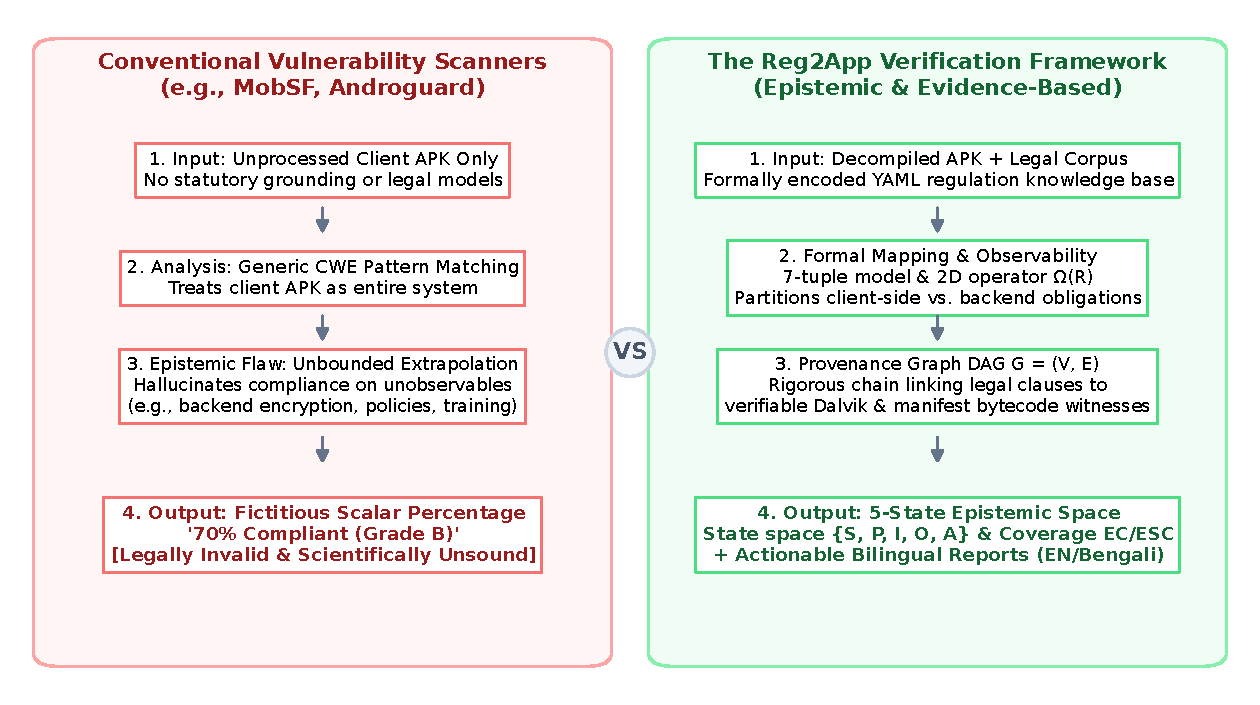
\includegraphics[width=0.85\textwidth]{figures/fig1_motivating_comparison.pdf}
\caption{Architectural contrast between conventional automated scanners and the Reg2App evidence verification pipeline. Conventional scanners (left) commit the Epistemic Overreach Trap: by analyzing only client APK artifacts without legal boundaries, they report scalar compliance scores (e.g., ``70\% Compliant''). In contrast, Reg2App (right) introduces formal 7-tuple mappings, an explicit 2D Observability Operator $\Omega(R_i)$ tagging unobservable backend and organizational requirements, an Evidence Provenance Graph $G = (V, E)$, and a discrete 5-state epistemic assessment model producing bounded metrics ($EC$ and $ESC$) alongside actionable bilingual reports.}
\label{fig:motivating_comparison}
\end{figure*}

\subsection{The Failure of Conventional Automated Scanners}
\label{sec:motivating:failure}

When presented with these findings, existing scanning engines calculate a scalar compliance score by taking the ratio of detected vulnerabilities to an arbitrary weight table:
\begin{align}
\label{eq:motivating:score}
\text{Reported Score} &= \frac{10 - \text{Vulnerabilities}}{10} \times 100\% = 70.0\%
\end{align}
This approach commits significant epistemic overreach~\cite{fagin_epistemic_logic}. By assuming that unobserved requirements (such as backend database residency and off-device user consent agreements) are compliant, conventional tools hallucinate compliance. Furthermore, these scanners output generic warnings without AST call graphs connecting sensitive inputs to storage sinks, lack authoritative statutory citations, and output reports exclusively in English technical jargon, imposing linguistic friction on local engineering teams.

\subsection{How Reg2App Resolves the Dilemma}
\label{sec:motivating:resolution}

Figure~\ref{fig:motivating_comparison} illustrates how Reg2App resolves this dilemma via bounded assessment. First, for Clause 1 (BB-CSF Section 4.1.3.12), the Network Analyzer evaluates the application against central bank baselines, finding that the APK explicitly configures certificate pin hashes for the bank's gateway. Reg2App generates an Evidence Witness Node $e_1$ containing the cryptographic hash and assigns Clause 1 to $\mathbf{Supported}$. Second, for Clause 2 (Draft BD-PDPA Section 15), Reg2App traces data flow from user input sources to standard XML storage lacking \texttt{EncryptedSharedPreferences}, generating Witness Node $e_2$ and assigning Clause 2 to $\mathbf{PotentialNonConformance}$. Crucially, for Clause 3 (Draft BD-PDPA Section 23), Reg2App consults the observability metadata $\Omega(R_3)$, evaluating it deterministically as $\mathbf{NotObservable}$ because user consent logs and foreign server hosting reside off-device.

Finally, Reg2App computes two objective metrics:
\begin{align}
\label{eq:motivating:ec}
EC &= \frac{N_{\mathbf{S}} + N_{\mathbf{P}}}{N_{\text{Obs}}} = \frac{1 + 1}{2} = 1.000 \\
\label{eq:motivating:esc}
ESC &= \frac{N_{\mathbf{S}}}{N_{\mathbf{S}} + N_{\mathbf{P}}} = \frac{1}{1 + 1} = 0.500
\end{align}
Rather than claiming an arbitrary 70\% compliance score, Reg2App delivers a mathematically bounded, evidence-grounded assessment. It evaluates only observable requirements, explicitly isolates unobservable backend obligations without speculation, and outputs a localized Bengali report directly explaining the remediation under BD-PDPA Section 15.
